\documentclass[codesnippet]{jss}

\usepackage[utf8]{inputenc}
\usepackage{tikz}
\usepackage{natbib}

%%%%%%%%%%%%%%%%%%%%%%%%%%%%%%
%% declarations for jss.cls %%%%%%%%%%%%%%%%%%%%%%%%%%%%%%%%%%%%%%%%%%
%%%%%%%%%%%%%%%%%%%%%%%%%%%%%%

%% almost as usual
\author{		Michael C. Sachs\\Biometric Research Branch, Division of Cancer Treatment and Diagnosis,
National Cancer Institute		}

\title{\pkg{plotROC}: A Better Tool for Plotting ROC Curves}

%% for pretty printing and a nice hypersummary also set:
\Plainauthor{ Michael C. Sachs} %% comma-separated
\Plaintitle{plotROC: A Better Tool for Plotting ROC Curves} %% without formatting

\Shorttitle{\pkg{plotROC}: A Better Tool for Plotting ROC Curves} %% a short title (if necessary)
%% an abstract and keywords
\Abstract{
  Plots of the receiver operating characteristic (ROC) curve are
  ubiquitous in medical research. Designed to simultaneously display the
  operating characteristics at every possible value of a continuous
  diagnostic test, ROC curves are used in oncology to evaluate screening,
  diagnostic, prognostic and predictive biomarkers. I reviewed a sample of
  ROC curve plots from the major oncology journals in order to assess
  current trends in usage and design elements. My review suggests that ROC
  curve plots are often ineffective as statistical charts and that poor
  design obscures the relevant information the chart is intended to
  display. I describe my new \proglang{R} package that was created to
  address the shortcomings of existing tools. The package has functions to
  create informative ROC curve plots, with sensible defaults and a simple
  interface, for use in print or as an interactive web-based plot. A web
  application was developed to reach a broader audience of scientists who
  do not use \proglang{R}.
}
\Keywords{ROC curves; graphics; interactive; plots}
\Plainkeywords{ROC curves; graphics; interactive; plots} %% without formatting
%% at least one keyword must be supplied

%% publication information
%% NOTE: Typically, this can be left commented and will be filled out by the technical editor
%% \Volume{50}
%% \Issue{9}
%% \Month{June}
%% \Year{2012}
%% \Submitdate{2012-06-04}
%% \Acceptdate{2012-06-04}

%% The address of (at least) one author should be given
%% in the following format:
\Address{
    Michael C. Sachs\\
    9609 Medical Center Drive, MSC 9735\\
    Bethesda, MD 20892\\
    telephone: 240-276-7888  \\\email{michael.sachs@nih.gov}
}
%% It is also possible to add a telephone and fax number
%% before the e-mail in the following format:
%% Telephone: +43/512/507-7103
%% Fax: +43/512/507-2851

%% for those who use Sweave please include the following line (with % symbols):
%% need no \usepackage{Sweave.sty}

%% end of declarations %%%%%%%%%%%%%%%%%%%%%%%%%%%%%%%%%%%%%%%%%%%%%%%


\begin{document}

\section{Introduction}\label{introduction}

\subsection{About ROC curves}\label{about-roc-curves}

The Receiver Operating Characteristic (ROC) curve is used to assess the
accuracy of a continuous measurement for predicting a binary outcome. In
medicine, ROC curves have a long history of use for evaluating
diagnostic tests in radiology and general diagnostics. ROC curves
originated in the field of signal detection theory .

For a continuous measurement that I denote as \(M\), convention dictates
that a test positive is defined as \(M\) equalling or exceeding some
fixed threshold \(c\): \(M \geq c\). The goal of ROC analysis is to
evaluate the classification accuracy of \(M\) in reference to the binary
outcome \(D\), which takes possible values \(0\) (negative) or \(1\)
(positive). It is implicitly assumed that the subpopulation having
\(D = 1\) tends to have larger values of \(M\) compared to the
subpopulation with \(D = 0\). The classification accuracy of \(M\) can
be evaluated by considering the confusion matrix (Table \ref{confus}).
The confusion matrix cross-classifies the predicted outcome \(M \geq c\)
versus the true outcome \(D\). The four cells of the matrix correspond
to the possible classification outcomes: a true positive, a false
positive, a true negative, and a false negative. ROC analysis assesses
the trade-offs between the test's fraction of true positives versus the
false positives.

\begin{table}
\begin{tabular}{l|c|c|c}
\multicolumn{1}{c}{}&\multicolumn{2}{c}{$D$}&\\
\cline{2-3}
\multicolumn{1}{c|}{}&1&0&\multicolumn{1}{c}{Total}\\
\cline{2-3}
 $M \geq c$ & true positive & false positive & test positive\\
\cline{2-3}
 $M < c$ & false negative & true negative & test negative\\
\cline{2-3}
\multicolumn{1}{c}{Total} & \multicolumn{1}{c}{disease positive} & \multicolumn{1}{c}{disease negative} & \multicolumn{1}{c}{}\\
\end{tabular}
\caption{\label{confus} Confusion matrix illustrating the possible classification outcomes of a continuous test $M$ with threshold $c$ versus the true outcome $D$. }
\end{table}

Formally, for a fixed cutoff \(c\), the true positive fraction is the
probability of a test positive in the diseased population:

\[ TPF(c) = P\{ M \geq c | D = 1 \} \]

and the false positive fraction is the probability of a test positive in
the healthy population:

\[ FPF(c) = P\{ M \geq c | D = 0 \} \]

Since the cutoff \(c\) is not fixed in advance, one can plot the TPF
against the FPF for all possible values of \(c\). This is exactly what
the ROC curve is, a plot of \(FPF(c)\) on the \(x\) axis and \(TPF(c)\)
along the \(y\) axis as \(c\) varies. A useless test that is not
informative at all in regards to the disease status has
\(TPF(c) = FPF(c)\) for all \(c\). The ROC plot of a useless test is
thus the diagonal line. A perfect test that is completely informative
about disease status has \(TPF(c) = 1\) and \(FPF(c) = 0\) for at least
one value \(c\). If the assumption that support of \(M | D = 1\) is
greater than that of \(M | D = 0\) holds, then the ROC curve will lie in
the upper left quadrant above the diagonal line, however this may not be
the case in a particular sample.

Given a sample of test and disease status pairs,
\((M_1, D_1), \ldots, (M_n, D_n)\), I can estimate the ROC curve by
computing proportions in the diseased and healthy subgroups separately.
Specifically, given a fixed cutoff \(c\), an estimate of the \(TPF(c)\)
is

\[ \widehat{TPF(c)} = \frac{\sum_{i = 1}^n 1\{M_i \geq c\} \cdot 1\{D_i = 1\}}{\sum_{i=1}^n 1\{D_i = 1\}}, \]

where \(1\{\cdot\}\) is the indicator function. An estimate for
\(FPF(c)\) is given by a similar expression with \(D_i = 1\) replaced
with \(D_i = 0\). Calculating these proportions for \(c\) equal to each
unique value of the observed \(M_i\) yields what is known as the
empirical ROC curve estimate. The empirical estimate is a step function.
Other methods exist to estimate the ROC curve, such as the binormal
parametric estimate which can be used to get a smooth curve. There are
also extensions that allow for estimation with time-to-event outcomes
subject to censoring. For a more thorough reference on the methods and
theory surrounding ROC curves, I refer interested readers to
\citet{pepe2003statistical}.

A common way to summarize the value of a test for classifying disease
status is to calculate the area under the ROC curve (AUC). The greater
the AUC, the more informative the test. The AUC summarizes the
complexities of the ROC curve into a single number and therefore is
widely used to facilitate comparisons between tests and across
populations. It has been criticized for the same reason because it does
not fully characterize the trade-offs between false- and true-positives.

\subsection{Design considerations}\label{design-considerations}

The main purpose of visually displaying the ROC curve is to show the
trade-off between the FPF and TPF as the cutoff \(c\) varies. This can
be useful for aiding viewers in choosing an optimal cutoff for decision
making, for comparing a small number of candidate tests, and for
generally illustrating the performance of the test as a classifier. In
practice, once the FPF and TPF are computed for each unique observed
cutoff value, they can be plotted as a simple line chart or scatter plot
using standard plotting tools. This often leads to the unfortunate
design choice of obscuring the critical and useful third dimension, the
range of cutoff values \(c\).

Another key design element is the use of a diagonal guideline for
comparison. They allow observers to roughly estimate the area between
the diagonal and the estimated ROC curve, which serves as a proxy for
estimating the value of the test for classification above a useless
test. Likewise, gridlines inside the plotting region and carefully
selected axes allow for accurate assessment of the TPF and FPF at
particular points along the ROC curve. Many medical studies use ROC
curves to compare a multitude of candidate tests to each other. In those
cases, curves need to be distinguished by using different colors or line
types combined with a legend, or direct labels inside the plotting
region.

In the medical literature, FPF and TPF are usually referred to in terms
of the jargon sensitivity and specificity. Sensitivity is equivalent to
the true positive fraction. Specificity is 1 - FPF, the true negative
fraction. Sometimes, the FPF and TPF are incorrectly referred to as
rates, using the abbreviations FPR and TPR. These are probabilities and
their estimates are proportions, therefore I prefer the use of the term
fraction as opposed to rate.

\subsection{Existing plotting
software}\label{existing-plotting-software}

The ROC curve plot is, at the most basic level, a line graph. Therefore,
once the appropriate statistics are estimated, existing plotting
functions can be used to create an ROC curve plot. Viewers can identify
ROC plots through context, by observing the shape of the line, and
through the addition of axis labels, titles, legends, and so on. In my
review of the oncology literature, I observed plots with the distinctive
characteristics of the plotting functions from Microsoft Excel
\citep{excel}, \proglang{SAS} \citep{sas}, \proglang{SPSS} \citep{spss},
and the base \proglang{R} plotting functions \citep{arr}.

There are several \proglang{R} packages related to ROC curve estimation
that contain dedicated plotting functions. The \pkg{ROCR} package
\citep{rocr} plots the FPF \emph{versus} TPF, as usual, and then takes
the interesting approach of encoding the cutoff values as a separate
color scale along the ROC curve itself. A legend for the color scale is
placed along the vertical axis on the right of the plotting region. The
\pkg{pROC} package \citep{pROC} provides an option for plotting cutoff
labels (\code{print.thres = TRUE}) and is mainly focused on estimating
confidence intervals and regions for restricted ranges of the ROC curve.
The plotting methods therein use the base \proglang{R} plotting
functions to create nice displays of the curves along with shaded
confidence regions. My \pkg{plotROC} package uses the \pkg{ggplot2}
\citep{ggplot2} plotting library to create clear, informative ROC plots,
with interactive features for use on the web, and sensible defaults for
use in print.

\subsection{Motivation and Literature
Review}\label{motivation-and-literature-review}

Anyone giving a cursory look at any of the major medical journals is
likely to find at least one ROC curve plot. I sought to assess the usage
of ROC curve plots and to evaluate the design choices made in the
current oncology literature by conducting a small literature review. I
searched Pubmed for clinical trials or observational studies in humans
reported in major oncology journals for the past 10 years for the terms
``ROC Curve'' OR ``ROC Analysis'' OR ``Receiver operating characteristic
curve''. The search was conducted on October 8, 2014 and returned 54
papers. From those papers, 47 images were extracted and reviewed. The
exact specifications for the Pubmed query are available in the
manuscript source files.

Each image consisted of a single ROC curve plot or a panel of multiple
plots. Each plot was inspected manually for the following design
features: the number of curves displayed, the type of axis labels
(sensitivity/ 1 - specificity or true/false positive fractions),
presence or absence of grid lines, presence or absence of a diagonal
guide line, whether any cutpoints were indicated, the type of curve
label (legend or direct label), and presence of other textual
annotations such as the AUC. The numerical results of the survey are
summarized in Table \ref{table1}.

\begin{table}[ht]
\centering
\begin{tabular}{ll}
  \hline
 & Percent (count) \\ 
  \hline
Number of curves &  \\ 
  $\quad$1 & 19.6 (9) \\ 
  $\quad$2 & 43.5 (20) \\ 
  $\quad$3 & 10.9 (5) \\ 
  $\quad$4+ & 26.1 (12) \\ 
  $\quad$Average (SD) & 2.6 (1.5) \\ 
  Axis labels &  \\ 
  $\quad$FPF/TPF & 13.0 (6) \\ 
  $\quad$mixed & 2.2 (1) \\ 
  $\quad$none & 2.2 (1) \\ 
  $\quad$sens/spec & 82.6 (38) \\ 
  Diagonal Guide & 43.5 (20) \\ 
  Gridlines & 17.4 (8) \\ 
  Cutoffs indicated & 15.2 (7) \\ 
  AUC indicated & 50.0 (23) \\ 
  Curve Labels &  \\ 
  $\quad$direct & 10.9 (5) \\ 
  $\quad$legend & 63.0 (29) \\ 
  $\quad$none & 19.6 (9) \\ 
  $\quad$title & 6.5 (3) \\ 
   \hline
\end{tabular}
\caption{Results of a literature review of major oncology journals for ROC curve plots. The rows indicate the frequency and count of key design elements of an ROC curve plot. FPR = False positive rate; TPR = True positive rate; sens = Sensitivity; spec = Specificity; AUC = Area under the Curve} 
\label{table1}
\end{table}

The small minority of the figures make any attempt to indicate the
values of the test cutoffs, which is an integral component of the ROC
curve. I conjecture that this is mainly due to the use of default
plotting procedures in statistical software. The software, by default,
treats the ROC curve as a 2 dimensional object, obscuring the cutoff
dimension. Gridlines and direct labels are also somewhat out of the
ordinary. The absence of these features make accurate determination and
comparison of the values more difficult. Many of the plots included
large tables containing estimates and inference for AUCs, while the ROC
curves themselves, numerous and without clear labels or reference lines,
merely served as decoration. I aim to solve some of these problems by
providing an easy-to-use plotting interface for the ROC curve that
provides sensible defaults.

The panels of Figure \ref{figure1} illustrate the most common styles of
ROC curve plots, and the associated design elements. I favor the use of
gridlines and a diagonal reference line to facilitate accurate readings
off of the axes. Direct labels are preferred over legends because they
omit the additional cognitive step of matching line types or colors to
labels. My \pkg{plotROC} package additionally provides plotting of
cutoff values, which are displayed interactively with the web-based
output option, and direct labels for print use. Exact confidence regions
for points on the ROC curve are optionally calculated and displayed.
Additionally, I use axis scales adjusted to be denser near the margins 0
and 1. In medical applications, it is often necessary to have a very low
FPR (less than 10\%, for instance), therefore the smaller scales are
useful for accurately determining values near the margins. The next
section details the usage of the \pkg{plotROC} \proglang{R} package and
these features.

\begin{Schunk}
\begin{figure}
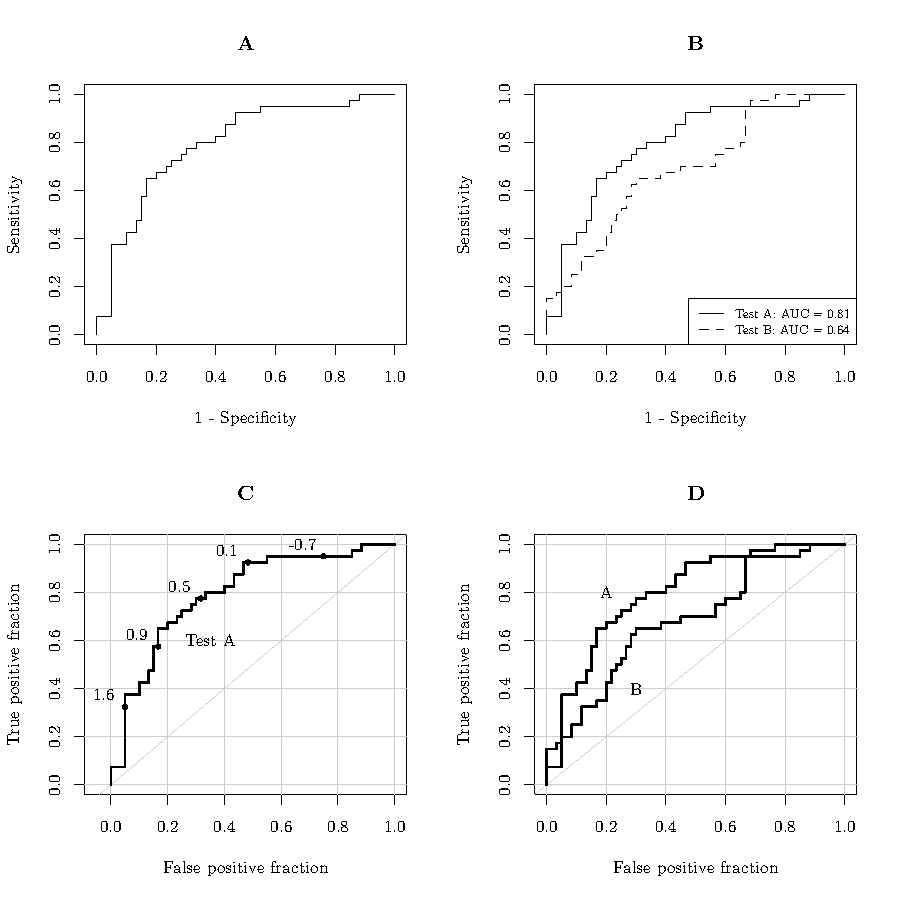
\includegraphics{figure/figure1-1} \caption[Illustration of design choices in plotting ROC curves]{Illustration of design choices in plotting ROC curves. Panel A shows a sparse ROC curve, with no design additions inside the plotting region. The plot results in more white space than anything else. It is difficult to accurately determine values without reference lines. Panel B shows a plot comparing 2 curves, with different line types and a legend. AUCs are also given in the legend. Panels C and D add gridlines, diagonal reference lines, and direct labels. \label{figure1}}\label{fig:figure1}
\end{figure}
\end{Schunk}

The vast majority of the figures that were reviewed looked more like
those in panels A and B than those in C and D. While plots like this do
technically display the trade-offs between false- and true-positives,
they minimize the amount of useful information that can be displayed in
the space needed to plot an ROC curve. The plots created by
\pkg{plotROC} attempt to increase the amount of information displayed in
ROC charts that would otherwise be mostly white space. This is useful
not only for print media, where space is limited, but also during data
analysis. The analyst can quickly and easily view information that would
otherwise be obscured by standard plotting software. The interactive
features take this one step further, enhancing the plots with high
density and easily accessible supplementary information.

\section{Usage of the package}\label{usage-of-the-package}

\subsection{Shiny application}\label{shiny-application}

I created a \pkg{shiny} application \citep{shiny} in order to make the
features more accessible to non-\proglang{R} users. A limited subset of
the functions of \pkg{plotROC} can be performed on an example dataset or
on data that users upload to the website. Resulting plots can be saved
to the users' machine as a pdf or as a stand-alone html file. It can be
used in any modern web browser with no other dependencies at the website
here: http://sachsmc.shinyapps.io/plotROC.

\subsection{Installation and loading}\label{installation-and-loading}

\pkg{plotROC} can be installed from the Comprehensive \proglang{R}
Archive Network, or installed from source.

\begin{Schunk}
\begin{Sinput}
R> install.packages("plotROC")
R> library(plotROC)
\end{Sinput}
\end{Schunk}

\subsection{Quick start}\label{quick-start}

After installing, the interactive Shiny application can be run locally.

\begin{Schunk}
\begin{Sinput}
R> shiny_plotROC()
\end{Sinput}
\end{Schunk}

\subsection{Command line basic usage}\label{command-line-basic-usage}

I start by creating an example data set. There are 2 markers, one that
is moderately predictive and one that is not as predictive.

\begin{Schunk}
\begin{Sinput}
R> set.seed(2529)
R> D.ex <- rbinom(200, size = 1, prob = .5)
R> M1 <- rnorm(200, mean = D.ex, sd = .65)
R> M2 <- rnorm(200, mean = D.ex, sd = 1.5)
R> 
R> test <- data.frame(D = D.ex, D.str = c("Healthy", "Ill")[D.ex + 1], 
+                    M1 = M1, M2 = M2, stringsAsFactors = FALSE)
\end{Sinput}
\end{Schunk}

\subsubsection{The Roc Geom}\label{the-roc-geom}

As of version 1.0.1, the \pkg{ggplot2} package \citep{ggplot2} exports
the previously internal functions \code{Geom} and \code{Stat}. This
enables developers to create their own statistical tranformations and
geometric layers, while enjoying all of the other features of
\pkg{ggplot2}. We have implemented the empirical ROC curve estimate and
the calculation of exact confidence regions as statistical
transformations: \code{stat_roc} and \code{stat_rocci}, respectively. We
have also defined geometric layers for the ROC curve and confidence
regions for the ROC curve: \code{geom_roc} and \code{geom_rocci},
respectively. For further discussion and details of the grammar of
graphics as implemented in \pkg{ggplot2}, we refer readers to
\citet{wickham2010layered} and the \pkg{ggplot2} vignettes.

To use the ROC geometric layer, I use the \code{ggplot} function to
define the aesthetic mappings, and the \code{geom_roc} function to add
an ROC curve layer. The \code{geom_roc} function requires the named
aesthetics \code{d} for disease status, and \code{m} for marker. By
default, the ROC geom and stat are linked, so that when \code{geom_roc}
is called, \code{stat_roc} does the computation, and when
\code{stat_roc} is called, \code{geom_roc} is used to plot the layer.
The disease status need not be coded as 0/1, but if it is not,
\code{stat_roc} assumes (with a warning) that the lowest value in sort
order signifies disease-free status.

\begin{Schunk}
\begin{Sinput}
R> basicplot <- ggplot(test, aes(d = D, m = M1)) + geom_roc()
\end{Sinput}
\end{Schunk}

The \code{geom_roc} layer includes the ROC curve line combined with
points and labels to display the values of the biomarker at the
different cutpoints. It accepts the argument \code{n.cuts} to define the
number of cutpoints to display along the curve. Labels can be supressed
by using \code{n.cuts = 0} or \code{labels = FALSE}, however points will
be displayed in the latter case. The size of the labels and the number
of significant digits can be adjusted with \code{labelsize} and
\code{labelround}, respectively.

\begin{Schunk}
\begin{Sinput}
R> ggplot(test, aes(d = D, m = M1)) + geom_roc(n.cuts = 0)
R> ggplot(test, aes(d = D, m = M1)) + geom_roc(n.cuts = 5, labelsize = 5, labelround = 2)
R> ggplot(test, aes(d = D, m = M1)) + geom_roc(n.cuts = 50, labels = FALSE)
\end{Sinput}
\end{Schunk}

\subsubsection{Confidence regions and the Rocci
Geom}\label{confidence-regions-and-the-rocci-geom}

It is common to compute confidence regions for points on the ROC curve
using the \citet{clopper1934use} exact method. Briefly, exact confidence
intervals are calculated for the \(FPF\) and \(TPF\) separately, each at
level \(1 - \sqrt{1 - \alpha}\). Based on result 2.4 from
\citet{pepe2003statistical}, the cross-product of these intervals yields
a \(100 * (1 - \alpha)\) percent rectangular confidence region for the
pair.

This is implemented in the \code{stat_rocci} and displayed as a
\code{geom_rocci} layer. These both require the same aesthetics as the
ROC geom, \code{d} for disease status and \code{m} for marker. By
default, a set of 3 evenly spaced points along the curve are chosed to
display confidence regions. Points corresponding to the confidence
regions are distiguished from the others with a different symbol. You
can select points by passing a vector of values in the range of \code{m}
to the \code{ci.at} argument. By default, the significance level
\(\alpha\) is set to 0.05, this can be changed using the
\code{sig.level} option. An example is shown in Figure \ref{ciex}.

\begin{Schunk}
\begin{Sinput}
R> basicplot + geom_rocci()
\end{Sinput}
\begin{figure}
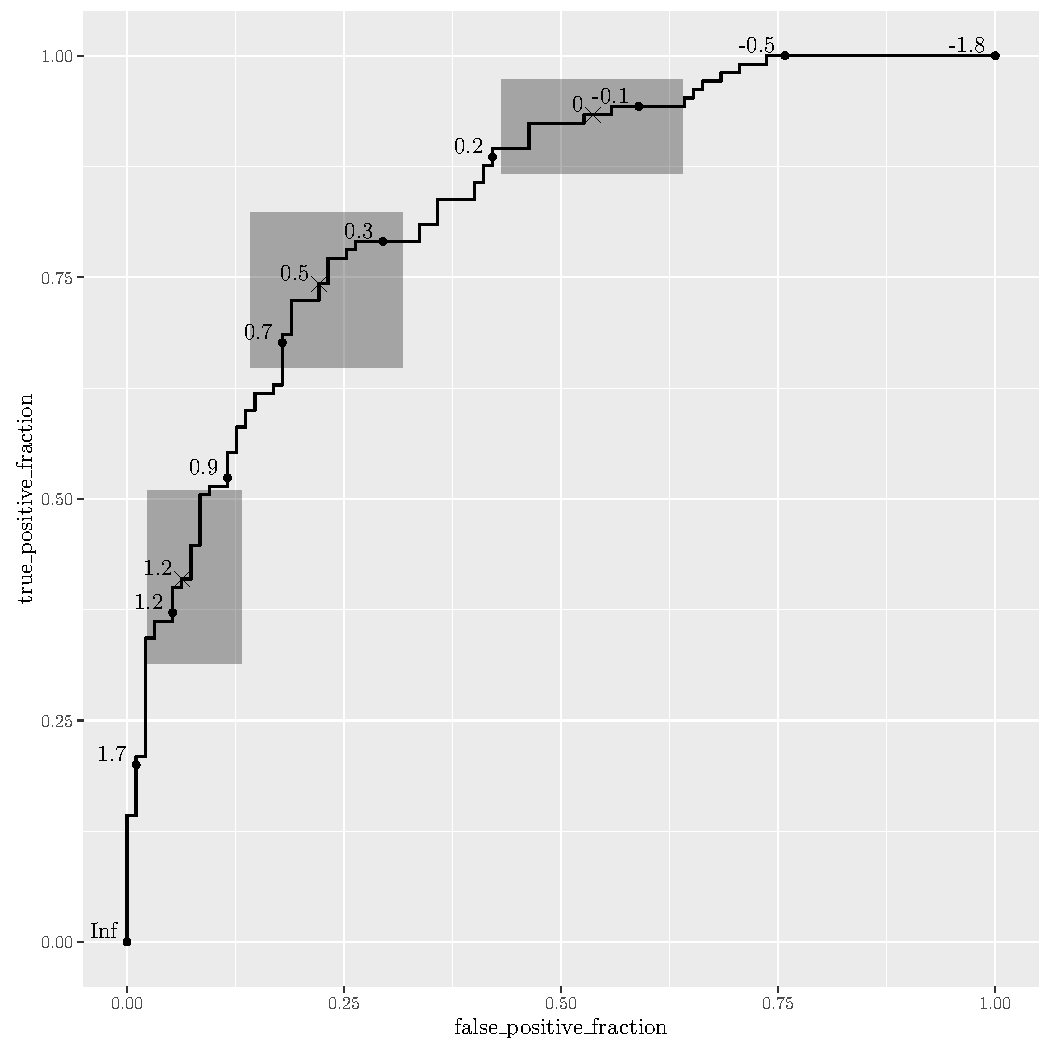
\includegraphics{figure/test-a-ci-1} \caption{Illustration of \pkg{plotROC} with exact confidence regions. \label{ciex}}\label{fig:test-a-ci}
\end{figure}
\begin{Sinput}
R> ## 
R> ## basicplot + geom_rocci(sig.level = .01)
R> ## ggplot(test, aes(d = D, m = M1)) + geom_roc(n.cuts = 0) +
R> ##   geom_rocci(ci.at = quantile(M1, c(.1, .4, .5, .6, .9)))
\end{Sinput}
\end{Schunk}

\subsubsection{Styles and Labels}\label{styles-and-labels}

The same objects like \code{basicplot} with Roc and/or Rocci layers can
be treated like any other ggplot objects. It can be printed to display
the figure, and other layers can be added to the plot. We provide the
function \texttt{style\_roc()} which is a layer containing a theme,
modified gridlines, and axes. Adding the \texttt{style\_roc()} layer to
the ggplot object creates a plot with sensible defaults for use in
print. This function has options for the number and location of major
and minor breaks, addition of the diagnoal guideline, axis labels, and
any theme object created for use with ggplot2 can be supplied.

The \code{direct_label} function takes a ggplot object as an argument
and annotates the figure with a direct label with a automatically chosen
location. It attempts to intellegently select an appropriate location
for the label, but the location can be adjusted with
\code{nudge_x, nudge_y} and \code{label.angle}. If the \code{labels}
argument is NULL, it will take the name from the mapped aesthetic. A
simple example with the default options is shown in Figure \ref{first}.

\begin{Schunk}
\begin{Sinput}
R> direct_label(basicplot) + style_roc()
\end{Sinput}
\begin{figure}
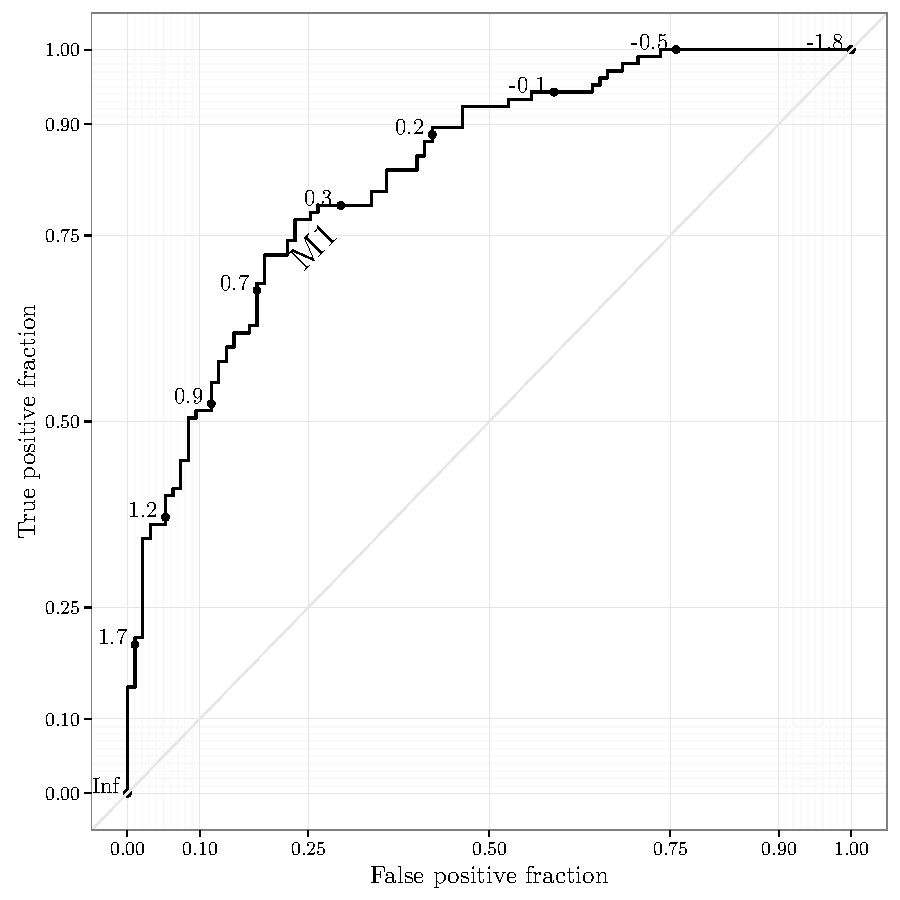
\includegraphics{figure/print-1} \caption{Illustration of ROC curve plot generated by \pkg{plotROC} for use in print. \label{first}}\label{fig:print}
\end{figure}
\begin{Sinput}
R> ## 
R> ## basicplot + style_roc(theme = theme_grey, xlab = "1 - Specificity")
R> ## direct_label(basicplot, labels = "Biomarker", nudge_y = -.1) + style_roc()
\end{Sinput}
\end{Schunk}

\subsubsection{Interactive ROC plots}\label{interactive-roc-plots}

The \code{basicplot} object, which is of class ggplot, can be used to
create an interactive plot and display it in the Rstudio viewer or
default web browser by passing it to the \code{plot_interactive_roc}
function. Give the function an optional path to an html file as an
argument called \code{file} to save the interactive plot as a complete
web page. A screen shot of an interactive plot is shown in Figure
\ref{interact}. Hovering over the display shows the cutoff value at the
point nearest to the cursor. Clicking makes the cutoff label stick until
the next click, and if confidence regions are available, clicks will
also display those as grey rectangles. By default,
\code{plot_interactive_roc} removes any existing Rocci geom and adds a
high-density layer of confidence regions. This can be suppressed by
using the \code{add.cis = FALSE} option. The points and labels layer of
the Roc geom can be hidden by using the \code{hide.points = TRUE}
option. Then, points and labels will be displayed only when the mouse is
hovering over the plotting region. Also by default, the \code{style_roc}
function is applied, the settings can be modified by passing a call to
that function.

\begin{Schunk}
\begin{Sinput}
R> plot_interactive_roc(basicplot)
R> plot_interactive_roc(basicplot, hide.points = TRUE)
R> plot_interactive_roc(basicplot, style = style_roc(theme = theme_bw()))
\end{Sinput}
\end{Schunk}

\begin{figure}[ht]
\centering
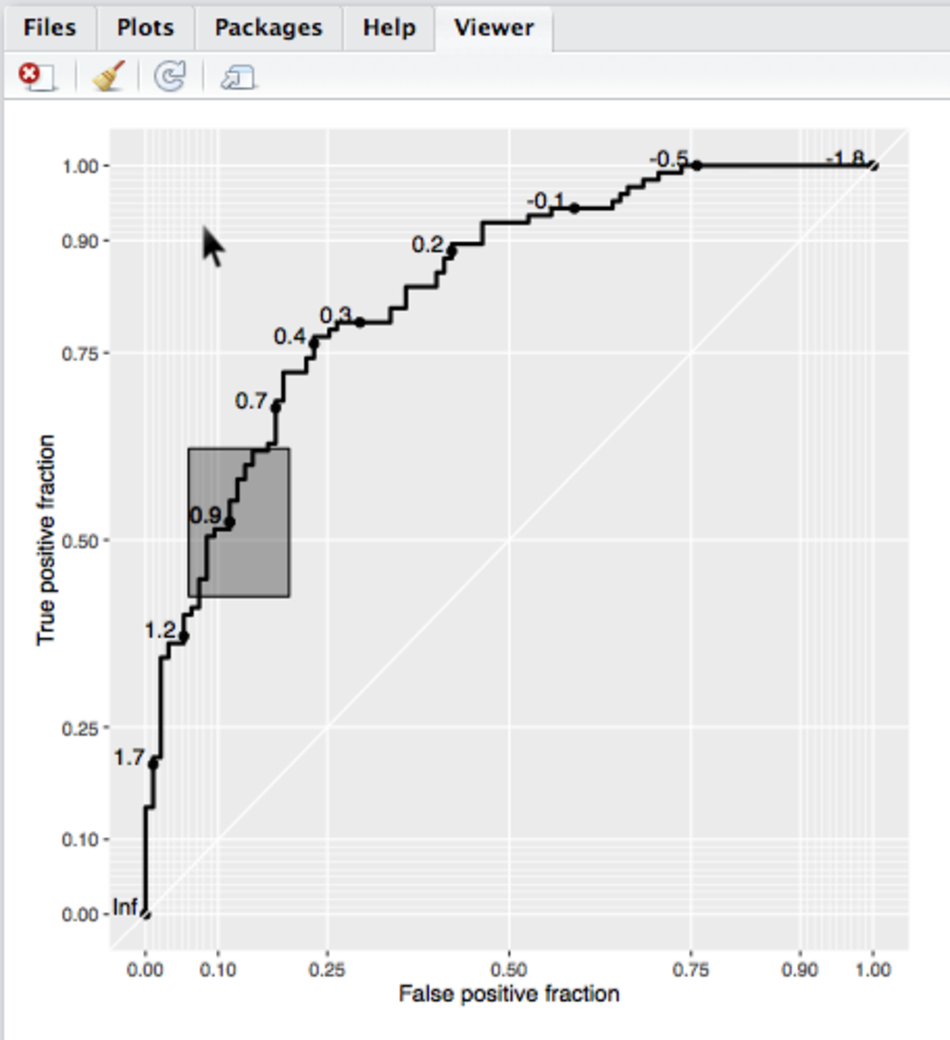
\includegraphics{figure/screen-shot.pdf}
\caption{Screen shot of an interactive plot created with \pkg{plotROC} being displayed in the Rstudio viewer. Hovering the mouse cursor over the plot causes the cutoff label nearest to the cursor to be displayed. Clicking will display a confidence region, if available, and make the label stick until the next click. For live examples, see the package vignette, or go to http://sachsmc.github.io/plotROC. \label{interact}}
\end{figure}

Hovering over the display shows the cutoff value at the point nearest to
the cursor. Clicking makes the cutoff label stick until the next click,
and if confidence regions are available, clicks will also display those
as grey rectangles. The confidence regions are automatically detected.
When the user clicks on the ROC curve, the confidence region for the TPF
and FPF is overlaid using a grey rectangle. The label and region stick
until the next click.

An interactive ROC plot can be exported by using the
\code{export_interactive_roc} function, which returns a character string
containing the necessary \proglang{HTML} and \proglang{JavaScript}. The
\proglang{JavaScript} source can be omitted by using the
\code{omit.js = TRUE} option. You may wish to do this when there are
multiple interactive figures in a single document; the source only needs
to be included once. The character string can be copy-pasted into an
html document, or better yet, incorporated directly into a dynamic
document using \pkg{knitr} \citep{knitr}. In a \pkg{knitr} document, it
is necessary to use the \code{cat} function on the results and use the
chunk options \code{results = 'asis'} and \code{fig.keep = 'none'} so
that the interactive plot is displayed correctly. For documents that
contain multiple interactive plots, it is necessary to assign each plot
a unique name using the \code{prefix} argument of
\code{export_interactive_roc}. This is necessary to ensure that the
\proglang{JavaScript} code manipulates the correct svg elements. For
examples of interactive plots and how to incorporate them into
\pkg{knitr} documents, see the package vignette
(\code{vignette("examples", package = "plotROC")}) or the web page
https://sachsmc.github.io/plotROC/. The next code block shows an example
\pkg{knitr} chunk that can be used in an .Rmd document to display an
interactive plot.

\begin{Code}
```{r int-no, results = 'asis', fig.keep = 'none'}
cat(
  export_interactive_roc(basicplot, 
                        prefix = "a")
  )
```
\end{Code}

\subsubsection{Multiple ROC curves}\label{multiple-roc-curves}

If you have grouping factors in your dataset, or you have multiple
markers measured on the same subjects, you may wish to plot multiple ROC
curves on the same plot. \pkg{plotROC} fully supports faceting and
grouping done by \pkg{ggplot2}. In out example dataset, we have 2
markers measured in a paired manner:

\begin{Schunk}
\begin{Sinput}
R> head(test)
\end{Sinput}
\begin{Soutput}
  D   D.str         M1          M2
1 1     Ill 1.48117155 -2.50636605
2 1     Ill 0.61994478  1.46861033
3 0 Healthy 0.57613345  0.07532573
4 1     Ill 0.85433197  2.41997703
5 0 Healthy 0.05258342  0.01863718
6 1     Ill 0.66703989  0.24732453
\end{Soutput}
\end{Schunk}

These data are in wide format, with the 2 markers going across 2
columns. \pkg{ggplot2} requires long format, with the marker result in a
single column, and a third variable identifying the marker. We provide
the convenience function \code{melt_roc} to perform this transformation.
The arguments are the data frame, a name or index identifying the
disease status column, and a vector of names or indices identifying the
the markers. Optionally, the names argument gives a vector of names to
assign to the marker, replacing their column names. The result is a data
frame in long format.

\begin{Schunk}
\begin{Sinput}
R> longtest <- melt_roc(test, "D", c("M1", "M2"))
R> head(longtest)
\end{Sinput}
\begin{Soutput}
    D          M name
M11 1 1.48117155   M1
M12 1 0.61994478   M1
M13 0 0.57613345   M1
M14 1 0.85433197   M1
M15 0 0.05258342   M1
M16 1 0.66703989   M1
\end{Soutput}
\end{Schunk}

Then, the dataset can be passed to the \code{ggplot} function, with the
marker name given as a grouping or faceting variable.

\begin{Schunk}
\begin{Sinput}
R> ggplot(longtest, aes(d = D, m = M, color = name)) + geom_roc() + style_roc()
R> ggplot(longtest, aes(d = D, m = M)) + geom_roc() + facet_wrap(~ name) + style_roc()
R> ggplot(longtest, aes(d = D, m = M, linetype = name)) + geom_roc() + geom_rocci()
R> ggplot(longtest, aes(d = D, m = M, color = name)) + geom_roc() + style_roc()
R> pairplot <- ggplot(longtest, aes(d = D, m = M, color = name)) + 
+   geom_roc(show.legend = FALSE) + style_roc()
R> direct_label(pairplot)
R> 
R> pairplot + geom_rocci()
R> pairplot + geom_rocci(linetype = 1)
\end{Sinput}
\end{Schunk}

Showing multiple curves is also useful when there is a factor that
affects the classification accuracy of the test. Let's create another
example dataset.

\begin{Schunk}
\begin{Sinput}
R> D.cov <- rbinom(400, 1, .5)
R> gender <- c("Male", "Female")[rbinom(400, 1, .49) + 1]
R> M.diff <- rnorm(400, mean = D.cov, sd = ifelse(gender == "Male", .5, 1.5))
R> 
R> test.cov <- data.frame(D = D.cov, gender = gender, M = M.diff)
\end{Sinput}
\end{Schunk}

\begin{Schunk}
\begin{Sinput}
R> bygend <- ggplot(test.cov, aes(d = D, m = M, color = gender)) + 
+   geom_roc(show.legend = FALSE)
R> direct_label(bygend) + style_roc()
\end{Sinput}
\begin{figure}
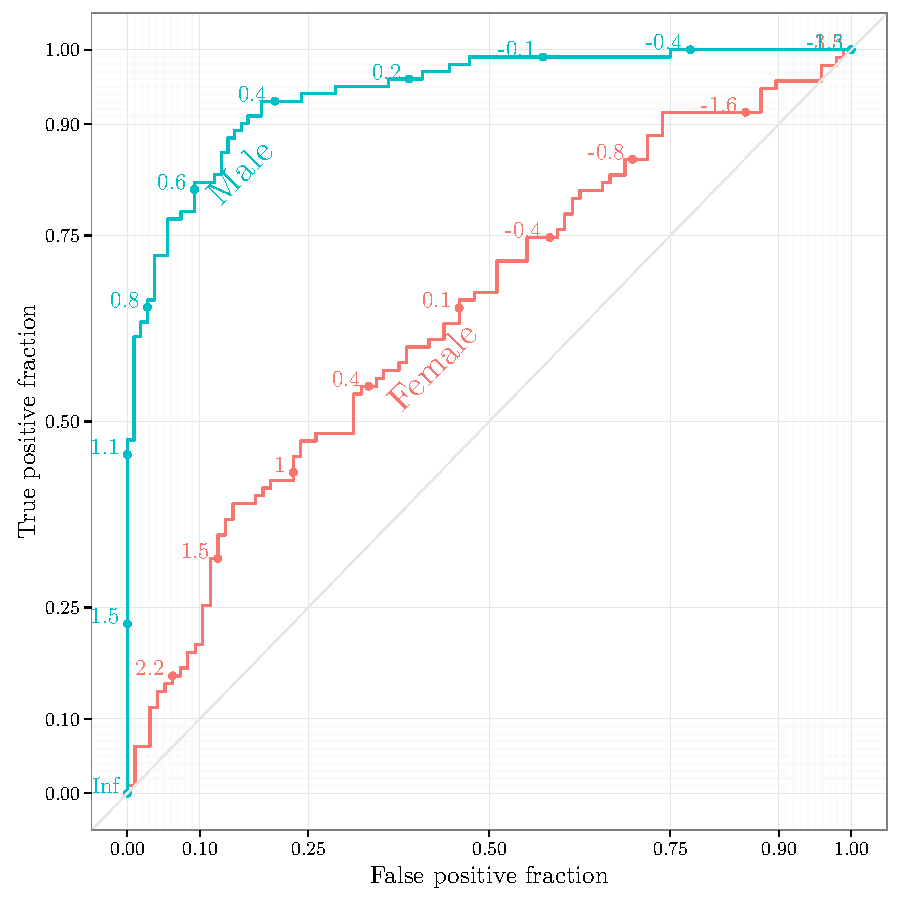
\includegraphics{figure/covplot-1} \caption{Illustration of \pkg{plotROC} with multiple curves. \label{multi}}\label{fig:covplot}
\end{figure}
\end{Schunk}

Interactive versions of the plots with grouping and faceting are fully
supported.

\subsection{Advanced options}\label{advanced-options}

\subsubsection{Themes and annotations}\label{themes-and-annotations}

\pkg{plotROC} uses the \pkg{ggplot2} package to create the objects to be
plotted. Therefore, themes and annotations can be added in the usual
\pkg{ggplot2} way. A \code{plot_journal_roc} figure with a new theme,
title, axis label, and AUC annotation is shown in Figure \ref{annotate}.
\pkg{plotROC} provides the convenience function \code{calc_auc} that
takes a ggplot object that has an Roc layer, extracts the data, and
calculates the AUC.

\begin{Schunk}
\begin{Sinput}
R> annotate <- basicplot + style_roc(theme = theme_grey) +
+   theme(axis.text = element_text(colour = "blue")) +
+   ggtitle("Themes and annotations") + 
+   annotate("text", x = .75, y = .25, 
+            label = paste("AUC =", round(calc_auc(basicplot)["AUC"], 2))) +
+   scale_x_continuous("1 - Specificity", breaks = seq(0, 1, by = .1))
\end{Sinput}
\end{Schunk}

\begin{Schunk}
\begin{figure}
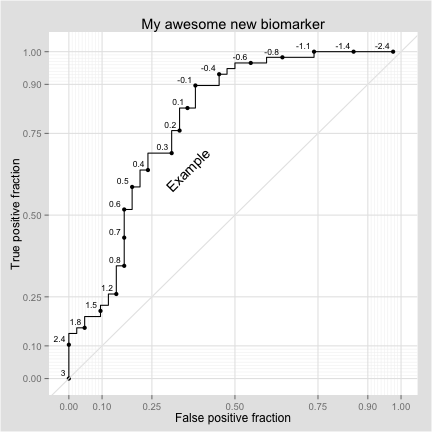
\includegraphics{figure/print2-1} \caption{Using \pkg{ggplot2} themes and annotations with \pkg{plotROC} objects. \label{annotate}}\label{fig:print2}
\end{figure}
\end{Schunk}

The results are compatible with all other \pkg{ggplot2} layers and
functions, and interactive versions are supported as long as there is an
Roc layer present.

\subsubsection{Other estimation methods}\label{other-estimation-methods}

By default \code{calculate_roc} computes the empirical ROC curve. There
are other estimation methods out there, as I have summarized in the
introduction. Any estimation method can be used, as long as the cutoff,
the TPF and the FPF are returned. Then you can simply pass those values
in a data frame to the \code{ggplot} function and override the default
statistical tranformation to \code{stat_identity}. For example, let us
use the binormal method to create a smooth curve. This approach assumes
that the test distribution is normal conditional on disease status.

\begin{Schunk}
\begin{Sinput}
R> D.ex <- test$D
R> M.ex <- test$M1
R> mu1 <- mean(M.ex[D.ex == 1])
R> mu0 <- mean(M.ex[D.ex == 0])
R> s1 <- sd(M.ex[D.ex == 1])
R> s0 <- sd(M.ex[D.ex == 0])
R> c.ex <- seq(min(M.ex), max(M.ex), length.out = 300)
R> 
R> binorm.roc <- data.frame(c = c.ex, 
+                              FPF = pnorm((mu0 - c.ex)/s0), 
+                              TPF = pnorm((mu1 - c.ex)/s1)
+                              )
R> 
R> binorm.plot <- ggplot(binorm.roc, aes(x = FPF, y = TPF, label = c)) + 
+   geom_roc(stat = "identity") + style_roc(theme = theme_grey)
\end{Sinput}
\end{Schunk}

The example is shown in Figure \ref{binorm}. Interactive plots with
\code{stat = 'identity'} are not currently supported.

\begin{Schunk}
\begin{Sinput}
R> binorm.plot
\end{Sinput}
\begin{figure}
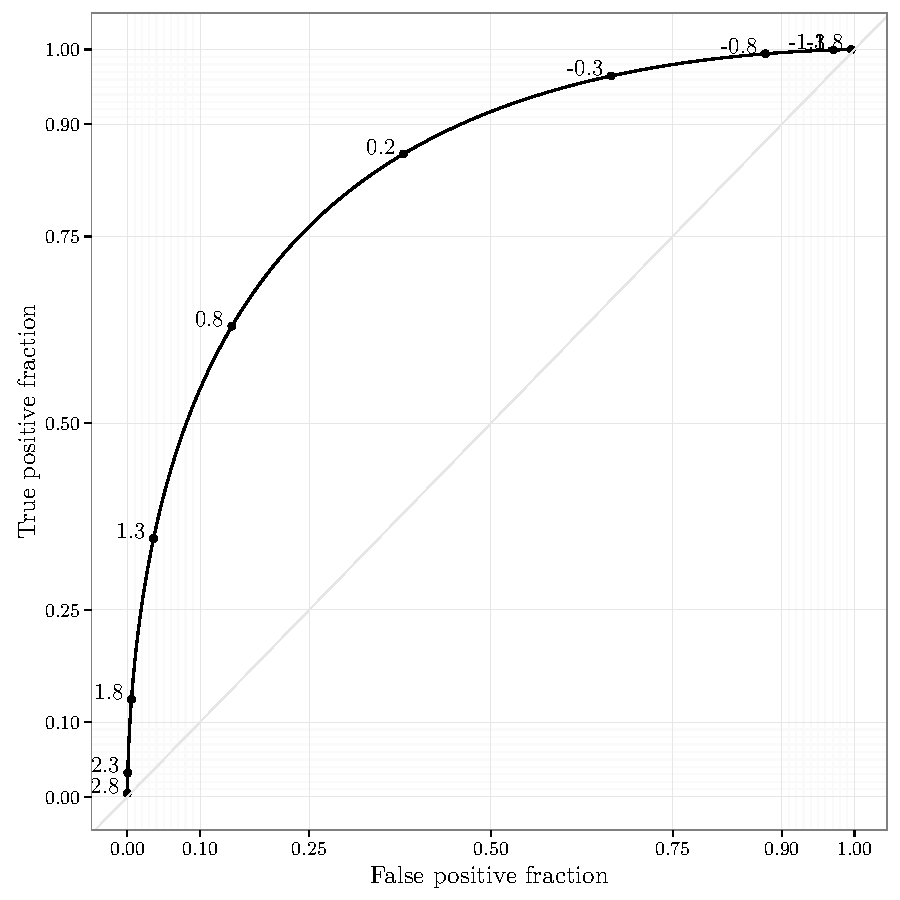
\includegraphics{figure/binormal-1} \caption[Illustration of smooth binormal ROC curve]{Illustration of smooth binormal ROC curve. \label{binorm}}\label{fig:binormal}
\end{figure}
\end{Schunk}

Another potential use of this approach is for plotting time-dependent
ROC curves for time-to-event outcomes estimated as desribed in
\citep{heagerty2000time}. Here is an example using the \pkg{survivalROC}
package \citep{survroc} for estimation:

\begin{Schunk}
\begin{Sinput}
R> library(survivalROC)
R> survT <- rexp(350, 1/5)
R> cens <- rbinom(350, 1, .1)
R> M <- -8 * sqrt(survT) + rnorm(350, sd = survT)
R> sroc <- lapply(c(2, 5, 10), function(t){ 
+   stroc <- survivalROC(Stime = survT, status = cens, marker = M, 
+                        predict.time = t, method = "NNE", 
+                        span = .25 * 350^(-.2))
+   data.frame(TPF = stroc[["TP"]], FPF = stroc[["FP"]], 
+              c = stroc[["cut.values"]], 
+              time = rep(stroc[["predict.time"]], 
+                         length(stroc[["FP"]])))
+   })
R> 
R> sroclong <- do.call(rbind, sroc)
R> 
R> survplot <- ggplot(sroclong, aes(x = FPF, y = TPF, label = c, color = time)) + 
+   geom_roc(labels = FALSE, stat = "identity")
\end{Sinput}
\end{Schunk}

\section{How it works}\label{how-it-works}

\pkg{plotROC} makes use of \pkg{ggplot2} \citep{ggplot2}, \pkg{gridSVG}
\citep{gridsvg}, and \pkg{d3.js} \citep{bostock2011d3} to create
interactive plots. The first step in the process is to create
\code{ggplot} objects with Roc and/or Rocci layers. They can be plotted
and inspected in the \proglang{R} console. These form the basis for both
the print versions and the interactive versions of the plots. Basic
styling and labeling can be added with the \code{style_roc} and
\code{direct_label} functions.

\pkg{plotROC} makes interactive plots by first converting the
\code{ggplot} object into a scalable vector graphic (svg) object with
the \code{gridSVG::grid.export} function. This function maps each
element of the plot to a corresponding element of the svg markup
language. I keep track of the names of the points and labels elements so
that I can add interactivity using \pkg{d3.js} and
\proglang{JavaScript}. The main interactive feature I wanted was to be
able to display the cutoff labels at the points on the ROC curve closest
to the mouse cursor.

There are many ways to solve this with \pkg{d3.js}, but I decided to use
Voronoi polygons to map the cursor location to the nearest point on the
ROC curve. The idea is that for the set of cutoff points along the ROC
curve, the \code{d3.geom.voronoi} function chain computes a set of
polygons overlaying the plotting region such that the area of each
polygon contains the region of the plot closest to it's corresponding
cutoff point. Hover events are bound to the polygons so that when the
mouse cursor moves around the plotting region, the closest point on the
ROC curve is made visible. Similarly, click events are bound to the
polygons so that the appropriate confidence region is made visible upon
clicking. The svg code and all necessary \proglang{JavaScript} code is
returned in the character string provided by
\code{export_interactive_roc}.

This approach is similar to what is done in the \pkg{gridSVG}
\code{grid.animate} function, which uses the svg \code{<animate />}
tags. However, the available features were not sufficient for my needs,
which is why I used \pkg{d3.js}. There are several other \proglang{R}
packages that aim to create interactive figures. The authors of
\pkg{animint} \citep{animint} created an extensive \proglang{JavaScript}
library that creates plots in a similar way as \pkg{ggplot2}. A set of
interactive features can be added to plots using \pkg{d3.js}.
\pkg{ggvis} \citep{ggvis}, \pkg{rCharts} \citep{rcharts}, and the more
recently released \pkg{htmlwidgets} \citep{htmlwidgets} all leverage
existing charting libraries written in \proglang{JavaScript}.
\pkg{qtlcharts} \citep{qtlcharts} uses a set of custom
\proglang{JavaScript} and \pkg{d3.js} functions to visualize data from
genetic experiments. Their general approach is to manipulate the data
and create options in \proglang{R}, and then let the charting libraries
or functions handle the rendering and interactivity. \pkg{plotROC} lets
\proglang{R} do the rendering, allowing the figures to be consistent
across print and web-based media, and retaining the distinctive
\proglang{R} style. This also allows users to manipulate the figures
directly in \proglang{R} to suit their needs, using tools that are more
accessible and familiar to most \proglang{R} users.

\section{Discussion}\label{discussion}

Here I have illustrated the usage and described the mechanics of a new
\proglang{R} package for creating ROC curve plots. The functions are
easy to use, even for non-\proglang{R} users \emph{via} the web
application, yet have sufficient flexibility to meet the needs of power
users. My approach to creating interactive plots differs from other
interactive charting packages. I found that existing approaches did not
meet the highly specialized needs of plotting ROC curves. While ROC
curve plots can technically be created with even the most basic plotting
tools, I find that specialized functions make the results clearer and
more informative. The functions are integrated into the existing and
popular \pkg{ggplot2} package, so that all the benefits and features
therein can be used effectively.

\subsection{Reproducibility note}\label{reproducibility-note}

This manuscript is completely reproducible using the source files. The
output below indicates the \proglang{R} packages and versions used.
Compiling the pdf output also requires \pkg{pandoc} version 1.13.1 and
\pkg{pdflatex}.

\begin{Schunk}
\begin{Sinput}
R> sessionInfo()
\end{Sinput}
\begin{Soutput}
R version 3.2.2 (2015-08-14)
Platform: x86_64-apple-darwin13.4.0 (64-bit)
Running under: OS X 10.10.5 (Yosemite)

locale:
[1] en_US.UTF-8/en_US.UTF-8/en_US.UTF-8/C/en_US.UTF-8/en_US.UTF-8

attached base packages:
[1] methods   stats     graphics  grDevices utils     datasets  base     

other attached packages:
[1] survivalROC_1.0.3  tikzDevice_0.8.1   plotROC_2.0.0     
[4] ggplot2_1.0.1.9003 xtable_1.7-4       stringr_1.0.0     
[7] knitr_1.11        

loaded via a namespace (and not attached):
 [1] Rcpp_0.12.1      digest_0.6.8     grid_3.2.2       plyr_1.8.3      
 [5] gtable_0.1.2     formatR_1.2.1    magrittr_1.5     evaluate_0.8    
 [9] scales_0.3.0     highr_0.5.1      stringi_0.5-5    labeling_0.3    
[13] tools_3.2.2      munsell_0.4.2    colorspace_1.2-6 filehash_2.3    
\end{Soutput}
\end{Schunk}


%\bibliographystyle{jss}
\bibliography{plotroc}


\end{document}
